\subsection{SVM}

\paragraph{}Una SVM es un algoritmo o clasificador de aprendizaje automático supervisado utilizado fundamentalmente para problemas de clasificación.
Dado un problema de aprendizaje automático supervisado de clasificación donde las instancias del problema pueden ser clasificadas en $N$ clases y un conjunto de ejemplos de entrenamiento de dicho problema, una SVM busca encontrar un hiperplano que los divida de manera lineal esas $N$ clases. De esta manera, frente a una nueva instancia del problema, la SVM será capaz de clasificarla generando una correspondencia entre esta instancia y una de las $N$ clases posibles.

\paragraph{}Se denominan vectores de soporte a aquellos ejemplos de entrenamiento más cercanos al hiperplano, la distancia entre el hiperplano y un vector de soporte se conoce como margen y para un conjunto de ejemplos de entrenamiento, SVM busca dividirlos de manera óptima con un hiperplano donde se maximice estos márgenes para cada uno de los vectores de soporte, cada uno asociado a su vez a una de las posibles clases de clasificación del problema. En un problema donde las instancias pueden ser clasificadas en dos clases, el hiperplano de dos dimensiones es representado por una línea recta y los vectores de soporte son aquellos ejemplos de entrenamiento más cercanos a ella, desde las dos direcciones posibles. La figura \ref{fig:svm_margin} muestra lo antedicho.

\textsc{\begin{figure}[ht!]
	\centering
    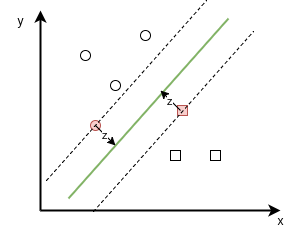
\includegraphics[width=.5\linewidth]{imagenes/svm_margenes.png}
	\caption{En esta figura se observan dos conjuntos de elementos (cuadrados y círculos), clasificados en dos clases, en base a dos características, \textit{x} e \textit{y}. El hiperplano generado por svm se muestra como la recta negra y se marcan los márgenes en lineas punteadas. Así, en color rojo se muestran los vectores de soporte, uno perteneciente a cada clase, siendo z la distancia entre cada vector de soporte y el hiperplano.}
	\label{fig:svm_margin}
\end{figure}}


\paragraph{}El hiperplano estará dado por la ecuación $g(\vec{x}) = \vec{w}^T\vec{x} + w_0$ donde $\vec{w}$ es un vector de pesos y $\vec{x}$ es el vector de características. La distancia a uno de los márgenes está dada por $z = \abs{g(\vec{x})} / \norm{\vec{w}} = 1 / \norm{\vec{w}}$, por lo que el margen total se computa como $1 / \norm{\vec{w}} +  1 / \norm{\vec{w}} = 2 / \norm{\vec{w}}$, así, minimizando la expresión $\norm{\vec{w}}$ se maximizan los márgenes, maximizando la separabilidad de las clases. 

\paragraph{}La confianza en la clasificación de una instancia del problema, estará dada por la distancia de dicho instancia al hiperplano de manera directamente proporcional.
La obtención de un hiperplano que divida de manera lineal a los ejemplos de entrenamiento no siempre es posible. Cuando no es posible se suele utilizar una técnica conocida como \textit{kernelización} para aumentar la dimensión del dominio donde se está buscando un hiperplano e, intentar obtener un hiperplano que separe linealmente a los ejemplos de entrenamiento en esa dimensión. De esta manera, es posible clasificar a nuevas instancias del problema de acuerdo a este nuevo hiperplano y transformar la clasificación obtenida a la dimensión original del problema dada por las clases de clasificación disponibles.

\paragraph{}Cuando se tienen más de dos clases objetivo para la clasificación, se utiliza un SVM Multiclase en el cual la técnica de prendizaje admite dos posibles estrategias. Por un lado \textit{One vs. Rest} (\textit{OVR}) y por otro \textit{One vs. One} (\textit{OVO}). Dado un conjunto de $N$ clases $\big\{c_1,c_2,\dots,c_N\big\}$, \textit{OVR} intentará clasificar $c_i$ contra ${c_1,c_2,\dots,c_(i-1),c_(i+1),\dots,c_N}$

\paragraph{}Entre las ventajas de utilizar SVM se encuentran que funciona correctamente en conjuntos de datos pequeños y limpios (con datos linealmente separables), resultando eficiente ya que utiliza un subconjunto de los ejemplos de entrenamiento únicamente, asociados a la definición del hiperplano. Las desventajas incluyen la poca efectividad que tienen en conjuntos de datos con ruido o clases diferenciadas de manera poco clara y que los tiempos de entrenamiento asociados pueden ser significativos para grandes conjuntos de entrenamiento.